\section{Bahan Bakar Minyak}
\label{sec:BBM-TP}

\subsection{Bensin}
\label{subsec:bensin-tp}

\begin{figure}[!ht]
    \centering
    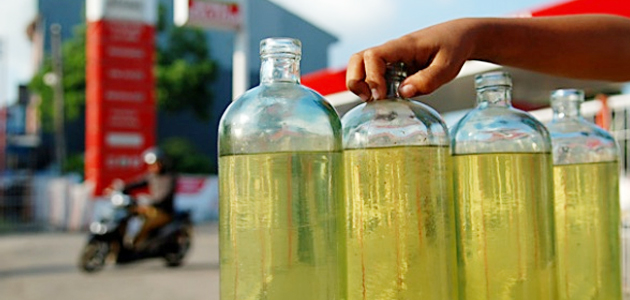
\includegraphics[width=0.6\textwidth,keepaspectratio]{gambar/BENSIN.jpg}
    \caption{Ilustrasi BBM Jenis Bensin}
    \label{fig:ilus-bensin}
\end{figure}

Bensin adalah cairan yang sangat mudah terbakar dan volatil yang terdiri dari hidrokarbon, yang terutama diproduksi melalui penyulingan minyak bumi. Bensin terutama digunakan sebagai bahan bakar untuk mesin penyala percikan, yang umum ditemukan pada mobil dan beberapa pesawat terbang. Properti penting yang mempengaruhi kinerja mesin termasuk volatilitasnya (diukur dengan tekanan uap Reid), angka oktan, dan kandungan panas. Tekanan uap Reid (RVP) adalah faktor penting dalam menentukan bagaimana bensin berfungsi di mesin \citep{Hsu_Robinson_2017}.

Peraturan lingkungan saat ini membatasi zat-zat yang berkontribusi pada pembentukan asap, melarang penggunaan tetraetil timbal (TEL), dan mengontrol tingkat sulfur, olefin, benzena, dan oksigenat dalam bensin. Bensin diproduksi di kilang dari berbagai bahan campuran menggunakan proses seperti distilasi minyak mentah, reformasi katalitik, pemecahan katalitik fluida (FCC), pemecahan termal, hidrokrediksi, alkilasi, isomerisasi, dan polimerisasi katalitik.

Untuk memastikan bensin memenuhi standar pasar, aditif sering kali ditambahkan untuk mencegah oksidasi dan korosi, menetralkan logam sisa, mengurangi penumpukan karbon pada katup masuk dan ruang pembakaran, serta menghindari pembentukan es di saat cuaca dingin \citep{Hsu_Robinson_2017}.

Bensin di Indonesia sebagian besar dipasok oleh PT. Pertamina (Persero) dengan nama Pertalite. Meskipun sekarang sudah banyak pemasok bahan bakar lain dari swasta namun pembelian bensin lewat SPBBU Pertamina masih disukai masyarakat karena mendapatkan subsidi dari Pemerintah.

\begin{figure}[!ht]
    \centering
    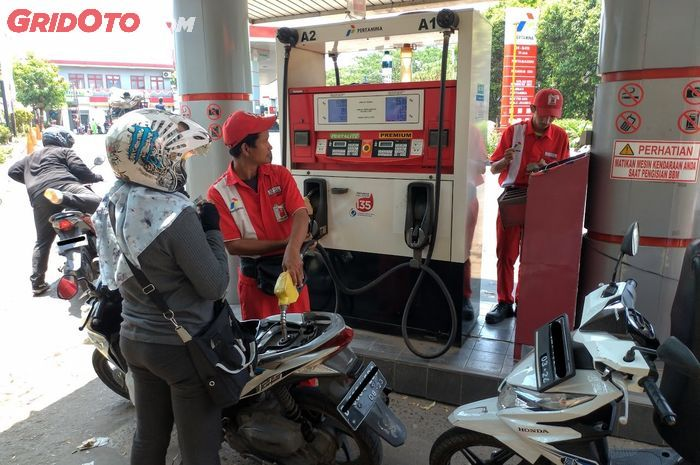
\includegraphics[width=0.7\textwidth]{gambar/isibensin.jpg}
    \caption{Ilustrasi Pengendara Motor Membeli Bensin di SPBU Pertamina (Gridoto.com)}
    \label{fig:ilus-isi-bensin}
\end{figure}

\subsection{Minyak Tanah}
\label{subsec:minyak-tanah-tp}

Minyak tanah telah menjadi bahan bakar rumah tangga yang penting sejak pertengahan abad ke-19, namun penggunaannya telah mengalami penurunan signifikan di negara-negara maju akibat elektrifikasi. Sebaliknya, negara-negara berkembang masih banyak menggunakan minyak tanah untuk memasak dan penerangan. Beberapa studi sudah menyoroti ketergantungan yang terus berlanjut pada minyak tanah di negara-negara berkembang, emisi yang dihasilkannya, dan bahaya terkait.

\begin{figure}[!ht]
    \centering
    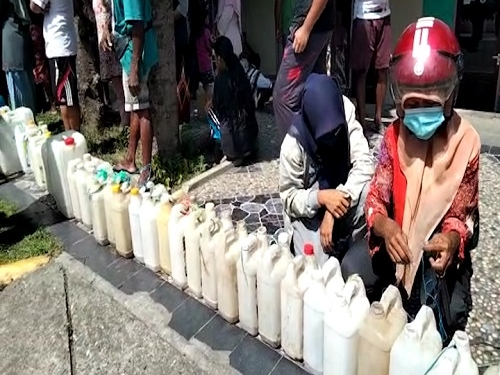
\includegraphics[width=0.65\textwidth]{gambar/Minyak-Berita-Maluku-Tengah-1-500x375.jpg}
    \caption{Potret Penduduk sedang Mengantri Minyak Tanah \citep{Radiodms_2021}}
    \label{fig:ilus-antri-minyak-tanah}
\end{figure}

Minyak tanah sering dianggap sebagai alternatif yang lebih bersih dibandingkan dengan bahan bakar padat seperti biomassa dan batu bara untuk memasak, dan umumnya digunakan dalam lampu di tempat-tempat yang tidak memiliki akses listrik. Sekitar 500 juta rumah tangga di seluruh dunia masih menggunakan minyak tanah untuk penerangan. Namun, penelitian tentang dampaknya masih terbatas dan tidak konsisten. Bahaya yang diketahui dari minyak tanah termasuk keracunan, kebakaran, dan ledakan, dengan beberapa perangkat mengeluarkan tingkat partikel halus, karbon monoksida, oksida nitrogen, dan sulfur dioksida yang tinggi. Emisi ini dapat mengganggu fungsi paru-paru dan meningkatkan risiko penyakit menular, asma, dan kanker \citep{Lam_Smith_Gauthier_Bates_2012}.

Mengingat penggunaan yang luas dan potensi bahayanya, diperlukan lebih banyak studi epidemiologi. Pemerintah seharusnya mempertimbangkan untuk mempromosikan teknologi yang lebih bersih untuk memasak dan penerangan alih-alih melanjutkan subsidi minyak tanah.

Menanggapi hal tersebut sejak tahun 2007, pemerintah Indonesia telah berupaya untuk mengalihkan rumah tangga dari minyak tanah ke gas. Meskipun akses ke gas cukup mudah, beberapa rumah tangga urban di Indonesia masih terus menggunakan minyak tanah untuk memasak. Salah satu daerah yang menjadi bukti nyata hal ini adalah Kabupaten Maluku Barat Daya. Data kuota BBM bersubsidi yang disalurkan oleh Pertamina untuk Kabupaten MBD menunjukkan bahwa sekitar 60\% dari BBM yang disalurkan adalah minyak tanah.

\begin{figure}[!ht]
    \centering
    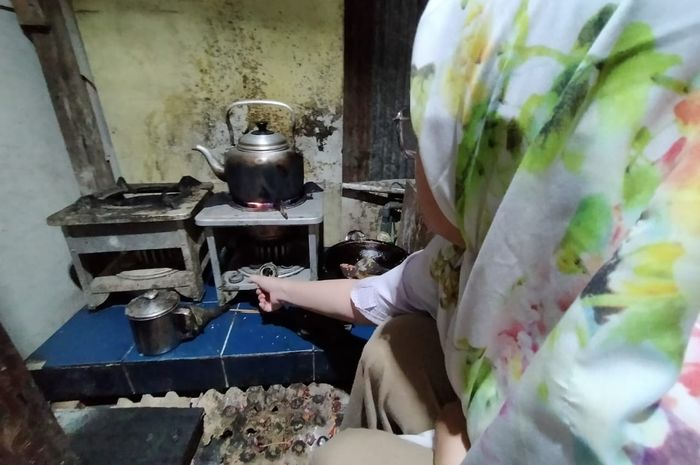
\includegraphics[width=0.65\textwidth]{gambar/masak-minyak-tanah.jpg}
    \caption{Penggunaan Minyak Tanah untuk Memasak \citep{Jumahudin_2021}}
    \label{fig:ilus-masak-minyak-tanah}
\end{figure}

Menurut data Susenas Maret 2018 dari BPS, terdapat 15.143 rumah tangga urban yang masih bergantung pada minyak tanah, dengan 80,20 persen di antaranya menggunakannya sebagai bahan bakar utama untuk memasak. Analisis regresi linier berganda mengungkapkan bahwa harga minyak tanah dan jenis kelamin kepala rumah tangga berdampak negatif terhadap intensitas penggunaan minyak tanah. Sebaliknya, pendapatan per kapita, usia kepala rumah tangga, jumlah anggota rumah tangga, dan tingkat pendidikan kepala rumah tangga berdampak positif terhadap intensitas penggunaan minyak tanah \citep{Soraya_Afiatno_2021}.


\subsection{Solar}
\label{subsec:solar-tp}

Bio Solar atau sekarang biasa dikenal dengan Biodiesel dapat diproduksi dari berbagai tanaman kaya minyak seperti kedelai, bunga matahari, dan kelapa, yang sering disebut sebagai RME (Rapeseed Methyl Ester). Proses esterifikasi adalah metode yang efisien biaya yang mengubah minyak nabati menjadi molekul yang mirip dengan hidrokarbon diesel, meskipun biodiesel tetap lebih mahal daripada diesel. Dengan sifat yang sangat mirip dengan bahan bakar diesel, biodiesel dapat digunakan dalam kendaraan diesel yang ada dan dicampur dengan diesel fosil dalam proporsi berapa pun. Meskipun memiliki kandungan energi sekitar 8\% lebih rendah dibandingkan diesel, biodiesel memiliki densitas yang lebih tinggi dan kualitas penyalaan yang lebih baik berkat angka cetane yang lebih tinggi \citep{Rifa’i_2020}.

Biodiesel, yang merupakan bahan bakar terbarukan dan biodegradable, juga dapat diproduksi dari minyak nabati, lemak hewan, atau lemak restoran daur ulang. Ini berfungsi sebagai alternatif yang lebih bersih daripada bahan bakar diesel dan memenuhi sifat-sifat utama yang diperlukan untuk bahan bakar mesin CI seperti yang diuraikan dalam Standar Bahan Bakar Terbarukan. Kinerja biodiesel dalam cuaca dingin tergantung pada rasio campuran dan bahan baku yang digunakan, dengan persentase biodiesel yang lebih rendah umumnya memiliki kinerja yang lebih baik pada suhu dingin.

\begin{figure}[!ht]
    \centering
    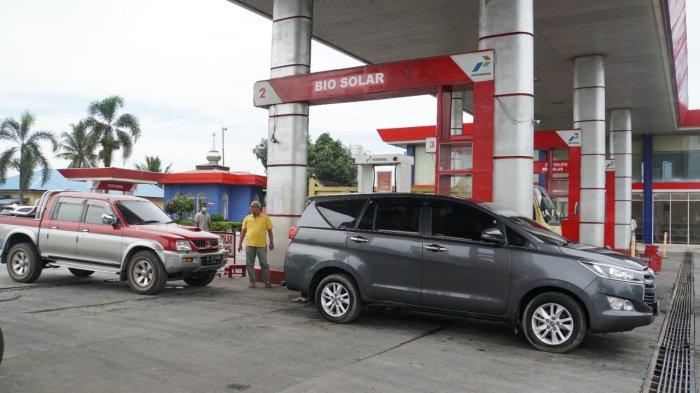
\includegraphics[width=0.75\textwidth]{gambar/mengisi-biosolar-di-spbu.jpg}
    \caption{Potret Salah Satu Stasiun Pengisian Bio Solar \citep{Rizky_2022}}
    \label{fig:ilus-beli-solar}
\end{figure}

Industri biodiesel berbasis minyak kelapa sawit nasional mengalami pertumbuhan signifikan pada tahun 2018, didorong oleh ekspansi program B20 ke sektor transportasi non-publik dan permintaan internasional yang tinggi. Permintaan domestik diperkirakan akan meningkat tajam di sektor transportasi dan manufaktur dalam beberapa tahun mendatang, sementara ekspor diperkirakan tetap kuat karena permintaan yang terus berlanjut dari UE dan China. Beberapa studi menunjukkan bahwa produksi biodiesel di Indonesia layak, dan para peneliti percaya bahwa biodiesel dapat digunakan baik sebagai bahan bakar tunggal maupun dicampur untuk digunakan dalam transportasi dan industri, termasuk bahan bakar untuk kapal nelayan dan mesin pertanian \cite{Rifa’i_2020}.
